% !TeX encoding = UTF-8

\chapter{ANÁLISE DOS RESULTADOS}\label{ch:resultados}
Este capítulo tem como finalidade apresentar os resultados obtidos através das implementações demonstradas no Capítulo 5.

\section{ANÁLISE DAS SÉRIES UTILIZADAS}
Após a implementação do modelo da RNA, através dos conjuntos de dados coletados, faz-se necessário avaliar como a respectiva técnica se comportou. Tendo isso em vista, a mesma foi aplicada em função do objetivo principal do trabalho, que é medir a capacidade de precisão de acerto no valor de abertura das ações. Portanto nas seções posteriores, será elaborada, de forma independente, uma análise de eficácia do modelo para o cenário de cada empresa utilizada no presente trabalho. É importante ressaltar que os modelos foram implementados levando em consideração toda a implementação dos \textit{scripts}, métodos e ferramentas utilizadas no Capítulo anterior.

\subsection{Análise do modelo da RNA: Intel Corporation}
A rede da Intel Corporation foi treinada com o objetivo de capturar o maior nível de variação possível dos dados, visando mapear um maior conjunto de padrões e, assim, responder de forma eficiente à dados dispersos através de uma boa capacidade de generalização. Tendo isso em vista, o período coletado foi de 09/04/2001 até 21/08/2017.


\begin{grafico}[h]
	\centering
	\fbox{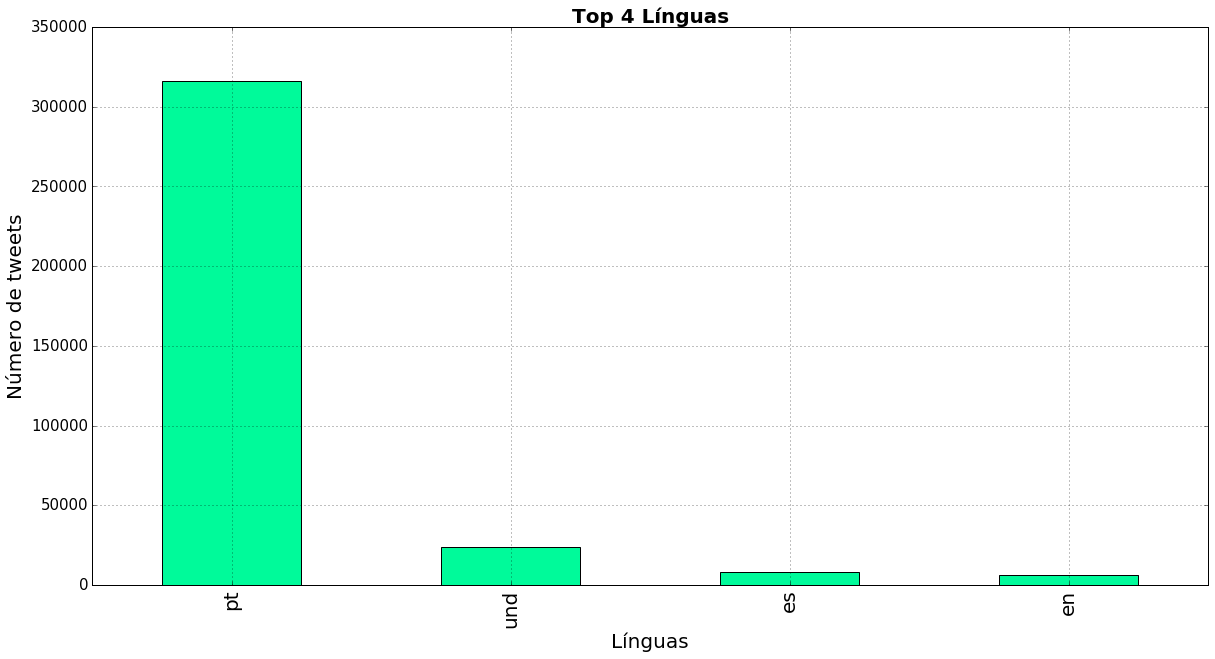
\includegraphics[width=1\textwidth]{linguas}}
	\caption{Idiomas que mais realizaram \textit{tweets}}
	\fonte{Elaborado pelo autor}
	\label{lingua}
\end{grafico}

\begin{table}[h]
\centering
\caption{Um nome qualquer}
\vspace{0.5cm}
\begin{tabular}{r|l|r}

Posição & País & IDH \\ % Note a separação de col. e a quebra de linhas
\hline                               % para uma linha horizontal
1 & Noruega        & .955 \\
2 & Austr{\'a}lia  & .938 \\
3 & EUA            & .937 \\
4 & Holanda        & .921 \\
5 & Alemanha       & .920            % não é preciso quebrar a última linha

\end{tabular}
\end{table}









